\documentclass[12pt,letterpaper]{exam}
\usepackage[lmargin=1in,rmargin=1in,tmargin=1in,bmargin=1in]{geometry}
\usepackage{../style/exams}

% -------------------
% Course & Exam Information
% -------------------
\newcommand{\course}{MATH 141: Exam 3}
\newcommand{\term}{Fall --- 2024}
\newcommand{\examdate}{11/20/2024}
\newcommand{\timelimit}{75 Minutes}

\setbool{hideans}{true} % Student: True; Instructor: False

% Shaded Lines - Area Between Curves
\usepgfplotslibrary{fillbetween}
%\usetikzlibrary{patterns}

% -------------------
% Content
% -------------------
\begin{document}

\examtitle
\instructions{Write your name on the appropriate line on the exam cover sheet. This exam contains \numpages\ pages (including this cover page) and \numquestions\ questions. Check that you have every page of the exam. Answer the questions in the spaces provided on the question sheets. Be sure to answer every part of each question and show all your work. If you run out of room for an answer, continue on the back of the page --- being sure to indicate the problem number.} 
\scores
\bottomline
\newpage


% -------------------
% Questions
% -------------------
\begin{questions}

% Question 1
\newpage
\question[15] Consider the plot of a function $f(x)$ given below.
	\[
	\fbox{
	\begin{tikzpicture}[scale=1.2,every node/.style={scale=0.5}]
	\begin{axis}[
	grid=both,
	axis lines=middle,
	ticklabel style={fill=blue!5!white},
	xmin= -1.5, xmax=12.5,
	ymin= -5.5, ymax=8.5,
	xtick={-2,0,...,12},
	ytick={-6,-4,...,8},
	minor tick = {-10,-9,...,12},
	xlabel=\(x\),ylabel=\(y\),
	]
	\addplot[line width= 0.03cm,samples=5,domain= 0:2] ({x},{3*x});
	\addplot[line width= 0.03cm,samples=5,domain= 2:4] ({x},{12 - 3*x});
	\addplot[line width= 0.03cm,samples=5,domain= 4:8] ({x},{-3});
	\addplot[line width= 0.03cm,samples=70,domain= 8:12] ({x},{sqrt(4 - (x - 10)^2) + 4});
	
	\addplot[holdot] coordinates{(4,0)(8,-3)};
	\addplot[soldot] coordinates{(4,-3)(8,4)};
	\end{axis}
	\end{tikzpicture}
	}
	\]
Using the above plot, compute the following: \par\vspace{0.3cm}
	\begin{enumerate}[(a)]
	\item $\displaystyle\int_0^8 f(x) \;dx=$ \vfill
	\item $\displaystyle\int_8^{12} f(x) \;dx=$ \vfill
	\item $\displaystyle\int_0^{12} f(x) \;dx=$ \vfill
	\item $\displaystyle\int_6^6 f(x) \;dx=$ \vfill
	\item The area between $f(x)$ and the $x$-axis. \vfill
	\end{enumerate}



% Question 2
\newpage
\question[10] Showing all your work, compute the following: \par\vspace{0.3cm}
	\begin{enumerate}[(a)]
	\item $\ds\int \left(\sin x - 5^x + 3 \tan x \right) \;dx$ \vfill
	\item $\ds\int_0^1 \left( \dfrac{1}{\sqrt{x}} - e^x \right) \;dx$ \vfill
	\end{enumerate}



% Question 3
\newpage
\question[10] Showing all your work, compute the following: \par\vspace{0.3cm}
	\begin{enumerate}[(a)]
	\item $\ds \dfrac{d}{dx} \int_{e^x}^\pi \dfrac{\arcsin(t)}{1 + t^2} \;dt$ \vfill
	\item $\ds \dfrac{d}{dx} \int_{-2}^{\sec(5x)} \ln \left( \dfrac{1 - t}{1 + t} \right) \;dt$ \vfill
	\end{enumerate}



% Question 4
\newpage
\question[10] Showing all your work, compute the following:
	\[
	\int \dfrac{dx}{5x^2 + 16}
	\]



% Question 5
\newpage
\question[10] Consider the region, $\mathcal{R}$, shown below.
	\[
	\fbox{
	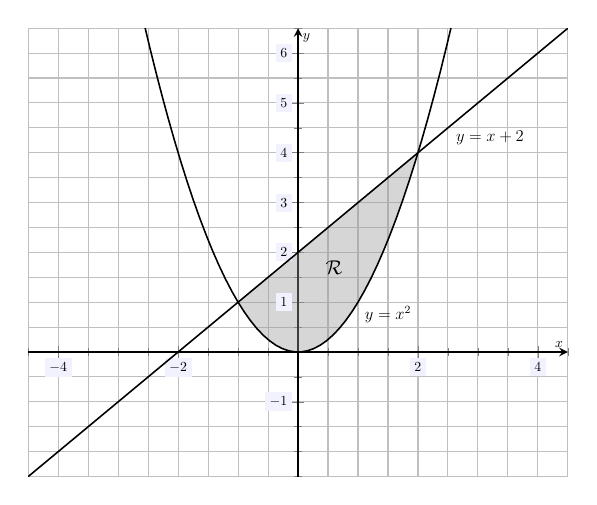
\begin{tikzpicture}[scale=1,every node/.style={scale=0.5}]
	\begin{axis}[
	grid=both,
	axis lines=middle,
	ticklabel style={fill=blue!5!white},
	xmin= -4.5, xmax=4.5,
	ymin= -2.5, ymax=6.5,
	xtick={-8,-6,...,8},
	ytick={-1,0,...,8},
	minor tick = {-8,-7.5,...,8},
	xlabel=\(x\),ylabel=\(y\),
	]
	\node at (1.5,0.75) {\large$y= x^2$};
	\addplot[name path=F,line width= 0.02cm,samples=5,domain= -10.5:10.5] ({x},{x + 2});
	\node at (3.2,4.3) {\large$y=x + 2$};
	\addplot[name path=G,line width= 0.02cm,samples=200,domain= -10.5:10.5] ({x},{x^2});
	\addplot[color=gray!80,opacity=0.4] fill between[of= F and G, soft clip={domain= -1:2}];
	\node at (0.6,1.7) {\Large$\mathcal{R}$};
	\end{axis}
	\end{tikzpicture}
	}
	\] 

\begin{enumerate}[(a)]
\item \scalebox{1}{Set-up \textit{but do not evaluate} an integral with respect to $x$ that computes the area of $\mathcal{R}$.} \vfill
\item \scalebox{1}{Set-up \textit{but do not evaluate} an integral with respect to $y$ that computes the area of $\mathcal{R}$.} \vfill
\end{enumerate}



% Question 6
\newpage
\question[10] Showing all your work, compute the following:
	\[
	\int_0^2 \dfrac{3x}{x^2 + 1} \;dx
	\]



% Question 7
\newpage
\question[15] Showing all your work, approximate the integral below using a left-hand sum with three evenly spaced rectangles \textit{but do not evaluate or simplify this sum}.
	\[
	\int_1^{13} \left( x \ln x - 1 \right) \;dx
	\]



% Question 8
\newpage
\question[10] Set-up \textit{but do not evaluate} an integral which computes the area between $f(x)= 3x + 4$ and $g(x)= 8 - x^2$.



% Question 9
\newpage
\question[10] Showing all your work, compute the following: \par\vspace{0.3cm}
	\begin{enumerate}[(a)]
	\item $\ds\int_{\pi/4}^{\pi/2} \cot x \csc x \;dx$ \vfill
	\item $\ds\int \left( 3 \cos x - \dfrac{x^3 + 6\sqrt{x}}{\sqrt{x}} \right) \;dx$ \vfill
	\end{enumerate}


\end{questions}
\end{document}